\documentclass[a4paper, 11pt]{article}
\usepackage{lipsum} %This package just generates Lorem Ipsum filler text. 
\usepackage{fullpage} % changes the margin
\usepackage{mathpazo}
\usepackage{multicol}
\usepackage{graphicx, float}
\usepackage{enumerate}
\usepackage{pythonhighlight}
\usepackage{booktabs}
\usepackage{listings}
\usepackage[T1]{fontenc}
\usepackage[english]{babel}
\usepackage{amsmath,amsfonts,amsthm} % Math packages

\begin{document}
%Header-Make sure you update this information!!!!
\noindent
\large\textbf{Chapter 2} \hfill \textbf{Siyuan Feng (516030910575)} \\
\normalsize {\bf CS 391 Computer Networking} \hfill ACM Class, Zhiyuan College, SJTU\\
Prof.~{\bf Yanmin Zhu} \hfill Due Date: October 18, 2018\\
TA.~{\bf Haobing Liu} \hfill Submit Date: \today

\section*{P7}
\begin{enumerate}[a.]
	\item $t_{total} = TT_l + 3RTT_r$
	\item $t_{total} = TT_l + 3RTT_r$ (suppose RTT between other DNS servers is also $RTT_r$)
	\item Since the cache exists, the IP address can be sent to client directly from the local DNS server. $RTT_1 = RTT_2 = TT_l$
\end{enumerate}

\section*{P8}
Suppose the time of client send message to the server and get response is $RTT_0$.
\begin{enumerate}[a.]
	\item $T = TT_l + 3RTT_r + 2RTT_0 + 8*2RTT_0 = 18RTT_0 + TT_l + 3RTT_r$
	\item $T = TT_l + 3RTT_r + 2RTT_0 + 2*2RTT_0 = 6RTT_0 + TT_l + 3RTT_r$
	\item $T = TT_l + 3RTT_r + 2RTT_0 + 2RTT_0 = 3RTT_0 + TT_l + 3RTT_r$
\end{enumerate}	
\section*{P14}
    Because that the destination, no matter is a client or another SMTP server, may be offline or unable to receive message. The server must retry to transmit message until the destination receive the message.
\section*{P18}
\begin{enumerate}[a.]
	\item Whois database stores the registered users or assignees of an Internet resource, such as a domain name, an IP address block or an autonomous system.
	\item I use $Aliyun WHOIS$ to obtain two DNS server $GoogleDNS(8.8.8.8)$ and $OpenDNS(208.67.222.222)$.
	\item The screenshot is shown below. \newline 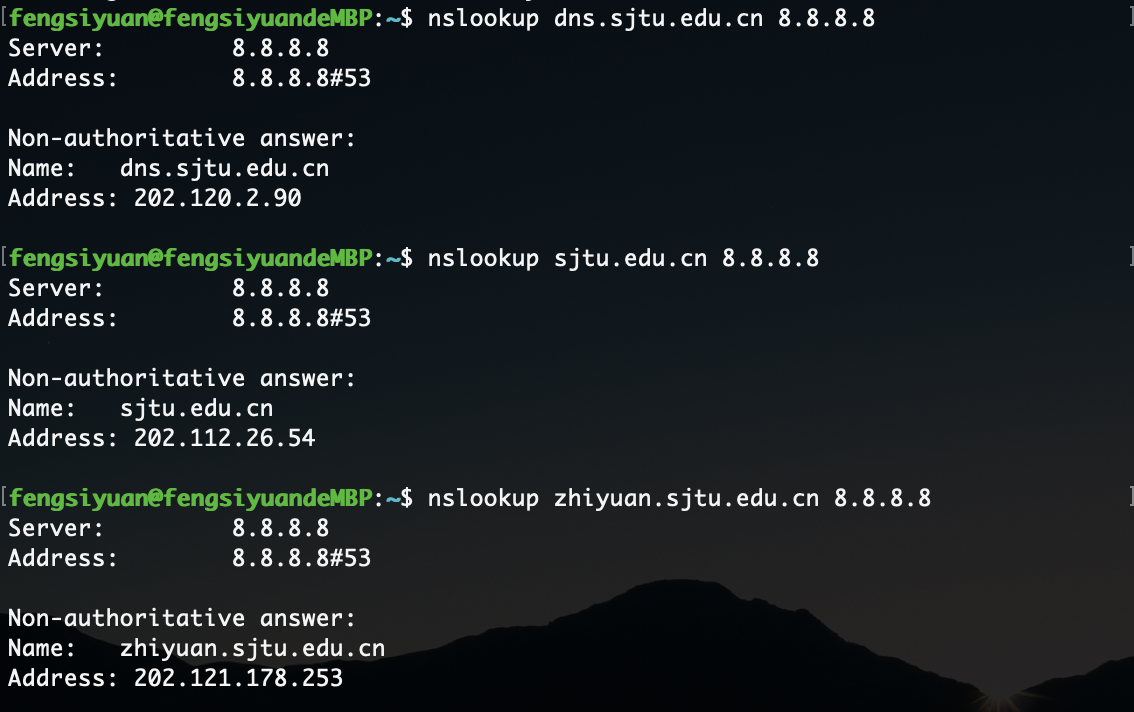
\includegraphics[width=\linewidth]{figure}
	\item Many popular website has multiply IP address, such as $www.baidu.com$.
	\item Ip range of SJTU is $202.120.0.0 - 202.120.63.255$, source from $APNIC$
 	\item An attacker can use the whois database and $nslookup$ tool to determine the IP address ranges, DNS server addresses, etc. for the target institution.
	\item If under an attack a victim can analyze the source address of packets, the victim can then use whois to obtain information about domain from which attack is coming and
possibly inform the administrators of the origin domain.
\end{enumerate}
\section*{P19}
	\begin{enumerate}[a.]
		\item The following delegation chain is used for www.sjtu.edu.cn
			\begin{enumerate}[1)]
				\item a.root-servers.net
				\item a.dns.cn
				\item dns.edu.cn
				\item dns.sjtu.edu.cn
				\item www.sjtu.edu.cn
			\end{enumerate}
		\item The following delegation chain is used for www.google.com
			\begin{enumerate}[1)]
				\item a.gtld-servers.net
				\item ns2.google.com
				\item www.baidu.com
			\end{enumerate}
	\end{enumerate}
\section*{P27}
	\begin{enumerate}[a.]
		\item If the TCP client runs before the server, the connection will be refused by server. Since there is a handshake protocol in TCP connection, which must be sent form a running server.
		\item If the TCP client runs before the server, no errors happened but the packets sent from the client will loss. After the server launches up, the connection will fully work.
		\item If the client try to connect server but with wrong port number, the same situation, as the server launches after the client, will happen.
	\end{enumerate}

\section*{P30}
\begin{itemize}
	\item For an application such as remote login (telnet and ssh), a byte-stream oriented protocols very natural since there is no notion of message boundaries in the application. When a user types a character, we simply drop the character into the TCP connection. 
	\item In other applications, we may be sending a series of messages that have inherent boundaries between them. For example, when one SMTP mail server sends another SMTP mail server several email messages back to back. Since TCP does not have a mechanism to indicate the boundaries, the application must add the indications itself, so that receiving side of the application can distinguish one message from the next. If each message were instead put into a distinct UDP segment, the receiving end would be able to distinguish the various messages without any indications added by the sending side of the application.
\end{itemize}
\end{document}
    